% !TeX spellcheck = en_US

\newgeometry{left=82.4mm,asymmetric}
\reversemarginpar
\fancyhfoffset[RO]{0mm}

\chapter[Curriculum Vitae]{Zacharias Steinmetz}

	\begin{cv}

	\info{\vspace*{0em}
		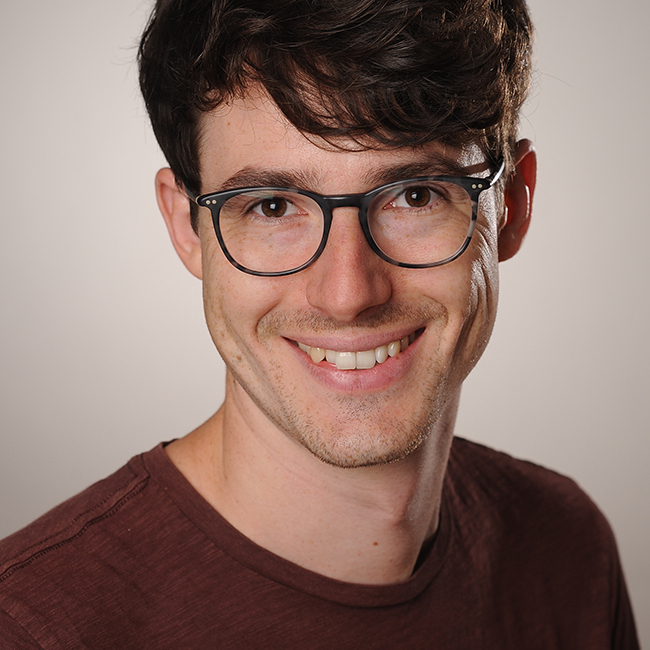
\includegraphics[width=.6\marginparwidth,,cfbox=black 0.75pt 0pt]{cv/portrait}}

	\vspace{.5em}

	\noindent
	\begin{minipage}{0.5\linewidth}
		Horststr. 157\\
		76829 Landau\\
		Germany
	\end{minipage}
	\begin{minipage}{0.5\linewidth}
		\begin{itemize}[left=.65em, noitemsep]
			\item[\color{InfRd}\envelope] \email{info@zsteinmetz.de}
			\item[\href{https://orcid.org/0000-0001-6675-5033}{\orcid}]
			\href{https://orcid.org/0000-0001-6675-5033}{0000-0001-6675-5033}
			\item[\href{https://publons.com/researcher/AAC-9025-2020/}{\publons}]
			\href{https://publons.com/researcher/AAC-9025-2020/}{AAC-9025-2020}
		\end{itemize}
	\end{minipage}

	\vspace{1em}
	\noindent Born September 23, 1989, in Frankfurt/Main \\
	\noindent Nationality: German

	\vspace{2em} % Extra white space


	%-------------------------------------------------------------------------------

	\heading{Education}

	\entry{10/2013--11/2016}{M.Sc. Ecotoxicology}{University of Koblenz--Landau (Germany)}
	\desc{\info{Thesis title}%
		``Tracking the transformation of phenolic compounds in soil with compound-specific stable carbon isotope analysis.''
		\newline
		\info{Final grade}1.2
	}

	\entry{10/2010--11/2013}{B.Sc. Environmental Sciences}{University of Koblenz--Landau (Germany)}
	\desc{\info{Thesis title}%
		``Persistence of chemical and biological effects of olive mill wastewater seasonally applied to loessial olive orchard soil.''
		\newline
		\info{Final grade}1.5
	}

	\entry{8/2000--7/2009}{Abitur}{Christian-Wirth-Gymnasium Usingen (Germany)}
	\desc{\info{Advanced courses}%
		Chemistry and mathematics
	}

	%-------------------------------------------------------------------------------

	\heading{Research and Work Experience}

	\entry{12/2016--present}{Research Associate}{University of Koblenz--Landau (Germany)}

	\desc{%
		Scrutinizing microplastic fate in agricultural soil using \ac{py-gc-ms}.
	}

	\entry{8/2019}{Guest Researcher}{LUT (Finland)}
	\desc{%
		Exchanging knowledge on microplastic extraction from soil and sediment and Raman spectroscopy.
	}

	\entry{4/2015--10/2015}{Student Employee}{RIFCON GmbH (Germany)}
	\desc{%
		Conducting individual-based ecological modeling and crop modeling in cooperation with Alterra (Netherlands).
	}

	\entry{6/2014--8/2014}{Intern}{MITOX Consultants/Eurofins (France)}
	\desc{%
		Assisting in ecotoxicological (semi-)field trials on non-target arthropods.
	}

	\entry{6/2013--8/2013}{Guest Researcher}{Agricultural Research Organization (Israel)}

	%-------------------------------------------------------------------------------

	\heading{Funding}

	\entry{}{Travel Grants \num{>1000} Euro}{}
	\desc{%
		%\info{5/2020}Ireland (University-intern research fund)\hfill{\small 550 Euro} \\
		\info{8/2019}Finland (Erasmus+)\hfill{\small 1895 Euro}\\
		\info{1/2018}Chile (Erasmus+)\hfill{\small 3020 Euro}
	}
	\entry{}{Scholarships}{}
	\desc{%
		\info{8/2016--12/2016}``AufLand'' publication grant for junior scientists\hfill{\small 3000 Euro}\\
		\info{3/2015--9/2016}\foreignlanguage{ngerman}{Studienstiftung des deutschen Volkes}\hfill{\small 7905 Euro}
	}

	%-------------------------------------------------------------------------------

	\heading{Teaching Experience}

	\entry{10/2021--present}{\foreignlanguage{ngerman}{Laborübungen Umweltanalytik}}{Co-supervisor}

	\entry{10/2017--present}{\foreignlanguage{ngerman}{Methoden der Natur- und Umweltwissenschaften}}{Associate lecturer}

	\entry{12/2016--present}{Advanced Environmental Chemistry}{Lecturer}

	\entry{10/2015--2/2016}{\texttt{R} for Beginners}{Teaching assistant}

	%-------------------------------------------------------------------------------

	\heading{Administrative Experience}

	\entry{12/2016--present}{Staff Representative}{University of Koblenz--Landau (Germany)}
	\desc{In various panels including the committee on educational affairs and the PhD committee of the faculty council of Environmental and Natural Sciences.}

	\entry{1/2014--12/2015}{Elected Student Representative}{University of Koblenz--Landau (Germany)}
	\desc{Faculty council of Environmental and Natural Sciences.}

	%-------------------------------------------------------------------------------

	\heading{Skills}

	\desc{\info{German}native
		\newline
		\info{English}proficient (10 school years, 1 year practice in the Philippines)
		\newline
		\info{French}basic (5 school years)
	}

	\desc{\info{Analytics}\Ac{py-gc-ms}, \ac{gc-ms}, GC/IRMS, GC/FID, HPLC, and \ac{ftir}--\ac{atr} using OpenChrom, Thermo Xcalibur, LCquan, and Isodat, Agilent ChemStation, and Open Specy for data analysis.
	}

	\desc{%
		\info{Computer skills}Advanced in \texttt{R} statistics and office applications
		\newline
		Competent in GIS (QGIS, GRASS), \textsc{python}, Linux shell, \LaTeX, git
		\newline
		Basic knowledge of Docker, SQL, HTML, and PHP.
		\newline

		\noindent\info{Software development}%
		Visit \href{https://github.com/zsteinmetz}{\faIcon{github} github.com/zsteinmetz} for an overview of my open-source software development.
	}

	%-------------------------------------------------------------------------------

	\heading{Selected Scientific Contributions}

	\desc{\small%
		\info{Peer-reviewed articles not listed in \nameref{ch:author-contributions}}
		\begin{refsection}[articles]
			\nocite{*}
			\printbibliography[heading=subbibliography,title=\vspace{-2.925\baselineskip}]
		\end{refsection}

		\vspace{.4\baselineskip}

		\noindent See \href{https://scholar.google.de/citations?user=klQROs4AAAAJ}{\googlescholar\ scholar.google.de/citations?user=klQROs4AAAAJ} for a complete publication list.

	}

	\desc{\small%
		\info{Referee}
		\textit{Journal of Analytical and Applied Pyrolysis}, \textit{Science of the Total Environment}, \textit{Environmental Pollution}, \textit{Polymers}, \textit{Frontiers in Environmental Science}.
	}

	\desc{%
		\info{Invited speaker}
		\begin{refsection}[talks]
			\nocite{*}
			\printbibliography[heading=subbibliography,title=\vspace{-2.925\baselineskip}]
		\end{refsection}
	}

	%-------------------------------------------------------------------------------

	\vspace{2em}

	\noindent
	\end{cv}

\normalmarginpar
\restoregeometry

\clearpage
\thispagestyle{empty}
\begin{fullwidth}
	~\vfill
	\centering\faIcon{jedi-order}
\end{fullwidth}
